\documentclass[tikz,border=4pt]{standalone}
\usepackage{amsmath,amssymb}
\usepackage[T1]{fontenc}
\usepackage{newtxtext,newtxmath}
\usetikzlibrary{arrows.meta,positioning,fit,backgrounds,calc}
\definecolor{ink}{HTML}{0B0B0B}
\definecolor{ink2}{HTML}{52514E}
\definecolor{blue}{HTML}{2A78D6}
\definecolor{bluel}{HTML}{CDE2FB}
\definecolor{orange}{HTML}{EB6834}
\definecolor{orangel}{HTML}{FBE0D3}
\definecolor{grayl}{HTML}{F0EFEC}
\begin{document}
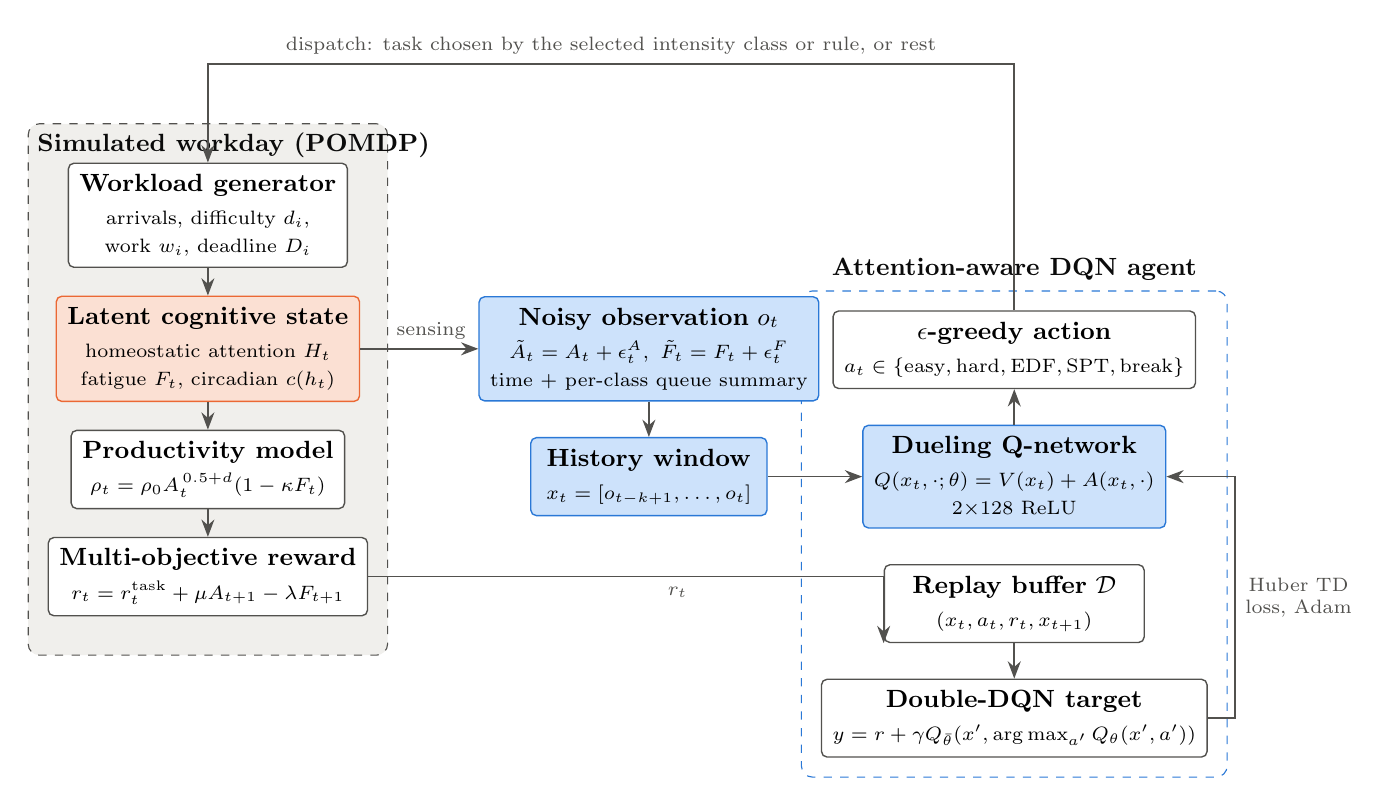
\begin{tikzpicture}[
  font=\small, >={Stealth[length=2.2mm]},
  box/.style={draw=ink2, rounded corners=2pt, align=center, inner sep=4pt, fill=white, line width=0.5pt},
  lat/.style={box, fill=orangel, draw=orange},
  obs/.style={box, fill=bluel, draw=blue},
  arr/.style={->, line width=0.6pt, draw=ink2},
  lab/.style={font=\scriptsize, text=ink2, align=center}
]
% ---------------- environment
\node[box, minimum width=3.2cm] (tasks) {\textbf{Workload generator}\\[1pt]\scriptsize arrivals, difficulty $d_i$,\\[-1pt]\scriptsize work $w_i$, deadline $D_i$};
\node[lat, below=0.35cm of tasks, minimum width=3.2cm] (cog) {\textbf{Latent cognitive state}\\[1pt]\scriptsize homeostatic attention $H_t$\\[-1pt]\scriptsize fatigue $F_t$, circadian $c(h_t)$};
\node[box, below=0.35cm of cog, minimum width=3.2cm] (eff) {\textbf{Productivity model}\\[1pt]\scriptsize $\rho_t=\rho_0 A_t^{\,0.5+d}(1-\kappa F_t)$};
\node[box, below=0.35cm of eff, minimum width=3.2cm] (rew) {\textbf{Multi-objective reward}\\[1pt]\scriptsize $r_t=r^{\text{task}}_t+\mu A_{t+1}-\lambda F_{t+1}$};
\begin{scope}[on background layer]
\node[fit=(tasks)(cog)(eff)(rew), draw=ink2, dashed, rounded corners=4pt, fill=grayl, inner sep=7pt, inner ysep=14pt,
      label={[font=\small\bfseries, text=ink, anchor=north west]north west:Simulated workday (POMDP)}] (env) {};
\end{scope}
% ---------------- observation
\node[obs, right=1.5cm of cog, minimum width=3.0cm] (o) {\textbf{Noisy observation} $o_t$\\[1pt]\scriptsize $\tilde A_t=A_t+\epsilon^A_t,\ \tilde F_t=F_t+\epsilon^F_t$\\[-1pt]\scriptsize time + per-class queue summary};
\node[obs, below=0.45cm of o, minimum width=3.0cm] (h) {\textbf{History window}\\[1pt]\scriptsize $x_t=[o_{t-k+1},\dots,o_t]$};
% ---------------- agent
\node[box, right=1.2cm of h, minimum width=3.3cm, fill=bluel, draw=blue] (q) {\textbf{Dueling Q-network}\\[1pt]\scriptsize $Q(x_t,\cdot;\theta)=V(x_t)+A(x_t,\cdot)$\\[-1pt]\scriptsize 2$\times$128 ReLU};
\node[box, above=0.45cm of q, minimum width=3.3cm] (pol) {\textbf{$\epsilon$-greedy action}\\[1pt]\scriptsize $a_t\in\{\text{easy},\text{hard},\text{EDF},\text{SPT},\text{break}\}$};
\node[box, below=0.45cm of q, minimum width=3.3cm] (buf) {\textbf{Replay buffer} $\mathcal D$\\[1pt]\scriptsize $(x_t,a_t,r_t,x_{t+1})$};
\node[box, below=0.45cm of buf, minimum width=3.3cm] (tgt) {\textbf{Double-DQN target}\\[1pt]\scriptsize $y=r+\gamma Q_{\bar\theta}(x',\arg\max_{a'}Q_\theta(x',a'))$};
\begin{scope}[on background layer]
\node[fit=(pol)(q)(buf)(tgt), draw=blue, dashed, rounded corners=4pt, inner sep=7pt,
      label={[font=\small\bfseries, text=ink]above:Attention-aware DQN agent}] (agent) {};
\end{scope}
% ---------------- arrows
\draw[arr] (cog.east) -- node[lab, above, pos=0.6]{sensing} (o.west);
\draw[arr] (o) -- (h);
\draw[arr] (h) -- (q);
\draw[arr] (q) -- (pol);
\draw[arr] (pol.north) -- ($(pol.north |- env.north)+(0,0.75)$) -- node[lab, above]{dispatch: task chosen by the selected intensity class or rule, or rest} ($(tasks.north |- env.north)+(0,0.75)$) -- (tasks.north);
\draw[arr] (tasks) -- (cog);
\draw[arr] (cog) -- (eff);
\draw[arr] (eff) -- (rew);
\draw[arr] (rew.east) -| node[lab, pos=0.3, below]{$r_t$} (buf.south west) ;
\draw[arr] (buf) -- (tgt);
\draw[arr] (tgt.east) -- ++(0.35,0) |- node[lab, pos=0.25, right]{Huber TD\\loss, Adam} (q.east);
\end{tikzpicture}
\end{document}
